%%%%%%%%%%%%%%%%%%%%%%%%%%%%%%%%%%%%%%%%%%%%%%%%%%%%%%%%%%%%%%%%%%%%%%%%%%%%%%%%%%%%%%%%%%%%%%%%%%%%%%%%%%%%%%%%%%%%%%%%%%%%%%%%%%%%%%%%%%%%%%%%%%%%%%%%%%%
% This is just an example/guide for you to refer to when submitting manuscripts to Frontiers, it is not mandatory to use Frontiers .cls files nor frontiers.tex  %
% This will only generate the Manuscript, the final article will be typeset by Frontiers after acceptance.                                                 %
%                                                                                                                                                         %
% When submitting your files, remember to upload this *tex file, the pdf generated with it, the *bib file (if bibliography is not within the *tex) and all the figures.
%%%%%%%%%%%%%%%%%%%%%%%%%%%%%%%%%%%%%%%%%%%%%%%%%%%%%%%%%%%%%%%%%%%%%%%%%%%%%%%%%%%%%%%%%%%%%%%%%%%%%%%%%%%%%%%%%%%%%%%%%%%%%%%%%%%%%%%%%%%%%%%%%%%%%%%%%%%

%%% Version 3.1 Generated 2015/22/05 %%%
%%% You will need to have the following packages installed: datetime, fmtcount, etoolbox, fcprefix, which are normally inlcuded in WinEdt. %%%
%%% In http://www.ctan.org/ you can find the packages and how to install them, if necessary. %%%

\documentclass[english]{frontiers/frontiersSCNS} % for Science, Engineering and Humanities and Social Sciences articles
%\documentclass{frontiersHLTH} % for Health articles
%\documentclass{frontiersFPHY} % for Physics and Applied Mathematics and Statistics articles

%\setcitestyle{square}
\usepackage{url,lineno,microtype}
\usepackage[colorlinks=true,linkcolor=black, citecolor=black!80, urlcolor=black!80]{hyperref}
\usepackage{doi}
\usepackage[onehalfspacing]{setspace}
\usepackage[toc,nomain,acronym,shortcuts,translate=false]{glossaries}

\def\keyFont{\fontsize{7}{9}\helveticabold }
\def\firstAuthorLast{Esteban {et~al.}} %use et al only if is more than 1 author
\def\Authors{Oscar Esteban\,$^{1,2,*}$, Emmanuel Caruyer\,$^{3}$, Alessandro Daducci\,$^{4}$, Meritxell Bach-Cuadra\,$^{4,5}$,%
M.-Jes\'us Ledesma-Carbayo\,$^{1,2}$ and Andres Santos\,$^{1,2}$}

\def\Address{%
$^{1}$Biomedical Image Technologies (BIT), ETSI Telecom., Universidad Polit\'ecnica de Madrid, Madrid, Spain \\
$^{2}$Centro de Investigaci\'on Biom\'edica en Red en Bioingenier\'ia, Biomateriales y Nanomedicina (CIBER-BBN), Spain \\
$^{3}$CNRS, IRISA (UMR 6074), VisAGeS research group, Rennes, France \\
$^{4}$Signal Processing Laboratory (LTS5), \'Ecole Polytechnique F\'ed\'erale de Lausanne (EPFL), Lausanne, Switzerland \\
${^5}$Dept. of Radiology, CIBM, University Hospital Center (CHUV) and University of Lausanne (UNIL), Lausanne, Switzerland %
}
% The Corresponding Author should be marked with an asterisk
% Provide the exact contact address (this time including street name and city zip code) and email of the corresponding author
\def\corrAuthor{Oscar Esteban}
\def\corrAddress{Biomedical Image Technologies (BIT), ETSI Telecomunicaci\'on, Av. Complutense 30, C203, E28040 Madrid, Spain}
\def\corrEmail{phd@oscaresteban.es}

% -*- root: main.tex -*-
% @Author: Oscar Esteban
% @Date:   2015-06-16 15:45:32
% @Last Modified by:   Oscar Esteban
% @Last Modified time: 2015-09-15 16:42:48

\newacronym{dmri}{dMRI}{diffusion MRI}
\newacronym{fa}{FA}{fractional anisotropy}
\newacronym{adc}{ADC}{anisotropic diffusion coefficient}
% \newacronym{hcp}{HCP}{Human Connectome Project}
\newacronym{fod}{FOD}{fiber orientation distribution}
\newacronym{fodf}{fODF}{fiber orientation distribution function}
\newacronym{wm}{WM}{white matter}
\newacronym{gm}{GM}{gray matter}
\newacronym{cgm}{cGM}{cortical gray matter}
\newacronym{dgm}{dGM}{deep gray matter}
\newacronym{csf}{CSF}{cerebrospinal fluid}
\newacronym{snr}{SNR}{signal-to-noise ratio}
\newacronym{csd}{CSD}{constrained spherical deconvolution}
\newacronym{cc0}{CC0}{Creative Commons Zero licence}
\newacronym{roc}{ROC}{receiver operating characteristic}
\newacronym{pve}{PVE}{partial volume effect}
\newacronym{cst}{CST}{corticospinal tract}
\newacronym{t1}{T1w}{T1-weighted}

\newglossaryentry{hcp}
{
	name={Human Connectome Project},
	text={HCP},
	first={Human Connectome Project (HCP, \cite{essen_human_2012})},
	long={Human Connectome Project},
	description={Human Connectome Project}
}

\newglossaryentry{bids}%
{
	name={BIDS},
	first={BIDS (Brain Imaging Data Structure, \cite{gorgolewski_brain_2015})},
	long={Brain Imaging Data Structure},
	description={Brain Imaging Data Structure}
}

\newglossaryentry{bedpostx}%
{
	name={BEDPOSTX},
	first={BEDPOSTX (Bayesian Estimation of Diffusion Parameters Obtained using Sampling Techniques modelling crossing --X-- fibres, \cite{jbabdi_modelbased_2012})},
	description={Bayesian Estimation of Diffusion Parameters Obtained using Sampling Techniques modelling crossing --X-- fibres}
}
\newacronym[first={FAST (FMRIB's Automated Segmentation Tool, \cite{zhang_segmentation_2001})}]%
{fast}{FAST}{FMRIB's Automated Segmentation Tool}
\newacronym[first={FIRST (FMRIB's Integrated Registration and Segmentation Tool, \cite{patenaude_bayesian_2011})}]%
{first}{FIRST}{FMRIB's Integrated Registration and Segmentation Tool}

\makeglossaries

\begin{document}

\onecolumn
\firstpage{1}

\title[Diffantom]{Diffantom: a software layer to build digital phantoms of whole-brain diffusion MRI}

\author[\firstAuthorLast ]{\Authors} %This field will be automatically populated
\address{} %This field will be automatically populated
\correspondance{} %This field will be automatically populated

\extraAuth{}% If there are more than 1 corresponding author, comment this line and uncomment the next one.
%\extraAuth{corresponding Author2 \\ Laboratory X2, Institute X2, Department X2, Organization X2, Street X2, City X2 , State XX2 (only USA, Canada and Australia), Zip Code2, X2 Country X2, email2@uni2.edu}


\maketitle

\linenumbers
\section*{Introduction}
The assessment of tractography from \gls*{dmri} data and subsequent analyses is challenging due to
  the lack of a gold standard.
Large efforts have been devoted to the development of physical phantoms
  \citep{lin_validation_2001,campbell_flowbased_2005,perrin_validation_2005,fieremans_simulation_2008,tournier_resolving_2008}.
\cite{cote_tractometer_2013} conducted a thorough review of tractography methodologies using the
  so-called \emph{FiberCup} phantom \citep{poupon_new_2008,fillard_quantitative_2011}.
These phantoms are appropriate to evaluate the resolution of fiber crossings and accuracy of
  direction-independent scalar parameters in very simplistic geometries.
Since the complexity of whole-brain tractography is unaccountable with current materials and proposed
  methodologies to build physical phantoms, digital simulations are increasingly popular.
Early digital phantoms started with simulation of simple geometries as well
  \citep{basser_in_2000,goessl_fiber_2002,tournier_limitations_2002,leemans_mathematical_2005}
  to evaluate resolution of fiber crossings.
These tools generally implemented the multi-tensor model \citep{alexander_analysis_2001,tuch_high_2002}
  to simulate fibers crossing, fanning, kissing, etc.
\cite{close_software_2009} presented the \emph{Numerical Fibre Generator}, a software to simulate
  spherical shapes filled with digital fiber-tracts.
\cite{caruyer_phantomas_2014} proposed \emph{Phantomas} to simulate any kind of analytic geometry
  inside a sphere.
\emph{Phantomas} models diffusion by a restricted and a hindered compartment, similar to
  \citep{assaf_composite_2005}.
\cite{wilkins_fiber_2014} proposed a whole-brain simulated phantom derived from voxel-wise orientation
  of fibers averaged from real \gls*{dmri} scans and the multi-tensor model with a compartment of
  isotropic-diffusion.
Recently, \cite{neher_fiberfox_2014} proposed \emph{FiberFox}, a visualization software to develop
  complex geometries and their analytical description.
Once the geometries are obtained, the software generates the corresponding \gls*{dmri} signal with a
  methodology very close to that implemented in \emph{Phantomas}.

In this paper we present \emph{Diffantom}, a software layer to generate diffusion phantoms at whole-brain
  scale and derived from real \gls*{dmri} datasets.
Particularly, we propose the \gls*{hcp} \citep{essen_human_2012} as the source of real data.
Finally, an example dataset is openly released along with all the necessary requirements and instructions
  to generate custom phantoms.


\section*{Data description}

\noindent\textbf{\textit{Data Generation\textcolon}}
The methods to generate the data in this paper are inspired by the work of \cite{wilkins_fiber_2014} and
  described in \autoref{fig:figure1}.
\emph{Diffantom} integrates two major improvements with respect to \citep{wilkins_fiber_2014}.
First, since we use a dataset from the \gls*{hcp} as input, data are corrected for the most relevant distortions.
\cite{wilkins_fiber_2014} explicitly state that their original data were not subjected to certain distortion
  corrections, and thus, generated data are affected correspondingly.
Second improvement is a more advanced signal model to generate the phantom using
  \emph{phantomas} \citep{caruyer_phantomas_2014}.
By default, diffusion data are generated using a scheme of 100 directions distributed in two shells with uniform
  coverage \citep{caruyer_design_2013}.
Custom schemes can be generated supplying the tables of corresponding $b$-vectors and $b$-values.
Rician noise is also included in \emph{phantomas}, and can be set by the user.
The default value for \gls*{snr} is pre-set to 90.0.

\noindent\textbf{\textit{Interpretation and use\textcolon}}
In order to release a reproducible dataset, along with an usable software to create custom data,
  we also distribute the software instrumentation presented in \autoref{fig:figure1}.
To ensure reproducibility and usability, the simulation pipeline is written using
  \emph{nipype} \citep{gorgolewski_nipype_2011}.
\autoref{fig:figure2}, block A, describes the recommended use case of \emph{diffantom} in the evaluation
  of algorithms and/or pipelines.
Finally, \autoref{fig:figure2}, blocks B1-3, show some tractograms of fundamental bundles to illustrate
  the features of the dataset.
To obtain the whole-brain tractogram, the example dataset underwent a simplified connectivity pipeline including
  \gls*{csd} and probabilistic tractography from
  \emph{MRTrix} \citep{tournier_mrtrix_2012}.
\Gls*{csd} was configured with up to 8 spherical harmonics, and tractography with 1.6$\times$10$^\text{6}$
  seed points evenly distributed across a dilated mask of the \gls*{wm} tissue.


\section*{Discussion and conclusion}

\noindent\textbf{\textit{Discussion\textcolon}}\label{sec:discussion} %
Whole-brain, realistic \gls*{dmri} phantoms are necessary in the developing field of structural
  connectomics.
The \emph{diffantom} is a derivative of \citep{wilkins_fiber_2014} in terms of methodology for
  simulation with two major improvements: the correctness of the \emph{minimally preprocessed} data
  \citep{glasser_minimal_2013} released within the \gls*{hcp}, and a more realistic diffusion
  model.
A possible competitor to \emph{diffantom} is the ground-truth data generated by the organizers of the
  Tractography Challenge held in the ISMRM 2015\footnote{\url{http://www.tractometer.org/ismrm_2015_challenge/}}.
Similarly to \emph{diffantom}, one \gls*{hcp} dataset is used as source of structural information.
However, in this case 25 fiber bundles were manually segmented to obtain a summary tractogram.
Then, making use of \emph{FiberFox}, the segmentation of each bundle is mapped to an analytical description
  which is feeded into \emph{phantomas}.
While this phantom is designed for the bundle-wise evaluation of tractography (with scores such as geometrical coverage,
  valid connections, invalid connections, missed connections, etc. \citep{cote_tractometer_2013}),
  \emph{diffantom} is intended for the connectome-wise evaluation of results, yielding tractography with
  a large number of bundles.
Therefore, \emph{diffantom} and \emph{FiberFox} are complementary as the hypotheses that can be investigated are different.
Moreover, \emph{diffantom} does not require costly manual segmentation of bundles, highly demanding in terms of physiology
  expertise and operation time.
This facilitates the use of \emph{diffantom} as a factory of whole-brain diffusion phantoms.
Lastly, since the gradient scheme can be set by the user, \emph{diffantom} can be seen as a mean to translate the so-called
  \emph{b-matrix} of the \gls*{hcp} to any target scheme.

\noindent\textbf{\textit{Conclusion\textcolon}}\label{sec:conclusion} %
\emph{Diffantom} is a software layer to be applied on \acrfull*{hcp} datasets, that is openly and freely distributed
  along with an example dataset.


\section*{Data Sharing}
The example dataset is available under the \gls*{cc0} in {\color{red} (dryad?)}.
Source code of \emph{diffantom} is available at \url{https://github.com/oesteban/phantomas} under an MIT licence.
\emph{Phantomas} is available in \url{https://github.com/ecaruyer/phantomas/} under the revised-BSD licence.

\section*{Disclosure/Conflict-of-Interest Statement}

The authors declare that the research was conducted in the absence of any commercial or financial relationships that could be construed as a potential conflict of interest.

\section*{Author Contributions}
All the authors contributed to this study.
OE designed the data generation procedure, implemented the processing pipelines and generated the example dataset.
EC implemented \emph{phantomas} \citep{caruyer_phantomas_2014}, helped integrate the project with the simulation routines.
OE, EC, AD thoroughtly discussed and framed the aptness of the data in the community.
AD, MBC, MJLC, and AS interpreted the resulting datasets.
MBC, MJLC, and AS advised on all aspects of the study.


\section*{Acknowledgments}
\textit{Funding\textcolon}
This study was supported by the Spanish Ministry of Science and Innovation
  (projects TEC-2013-48251-C2-2-R and INNPACTO XIORT), Comunidad de Madrid (TOPUS) and
  European Regional Development Funds, the Center for Biomedical Imaging
  (CIBM) of the Geneva and Lausanne Universities and the EPFL, as well as the
  Leenaards and Louis Jeantet Foundations.


\bibliographystyle{frontiers/frontiersinSCNS_ENG_HUMS}
%\bibliographystyle{frontiersinHLTH&FPHY} % for Health and Physics articles
\bibliography{Remote}

%%% Upload the *bib file along with the *tex file and PDF on submission if the bibliography is not in the main *tex file

\glsresetall

\section*{Figures}

\begin{figure}[h!]
\begin{center}
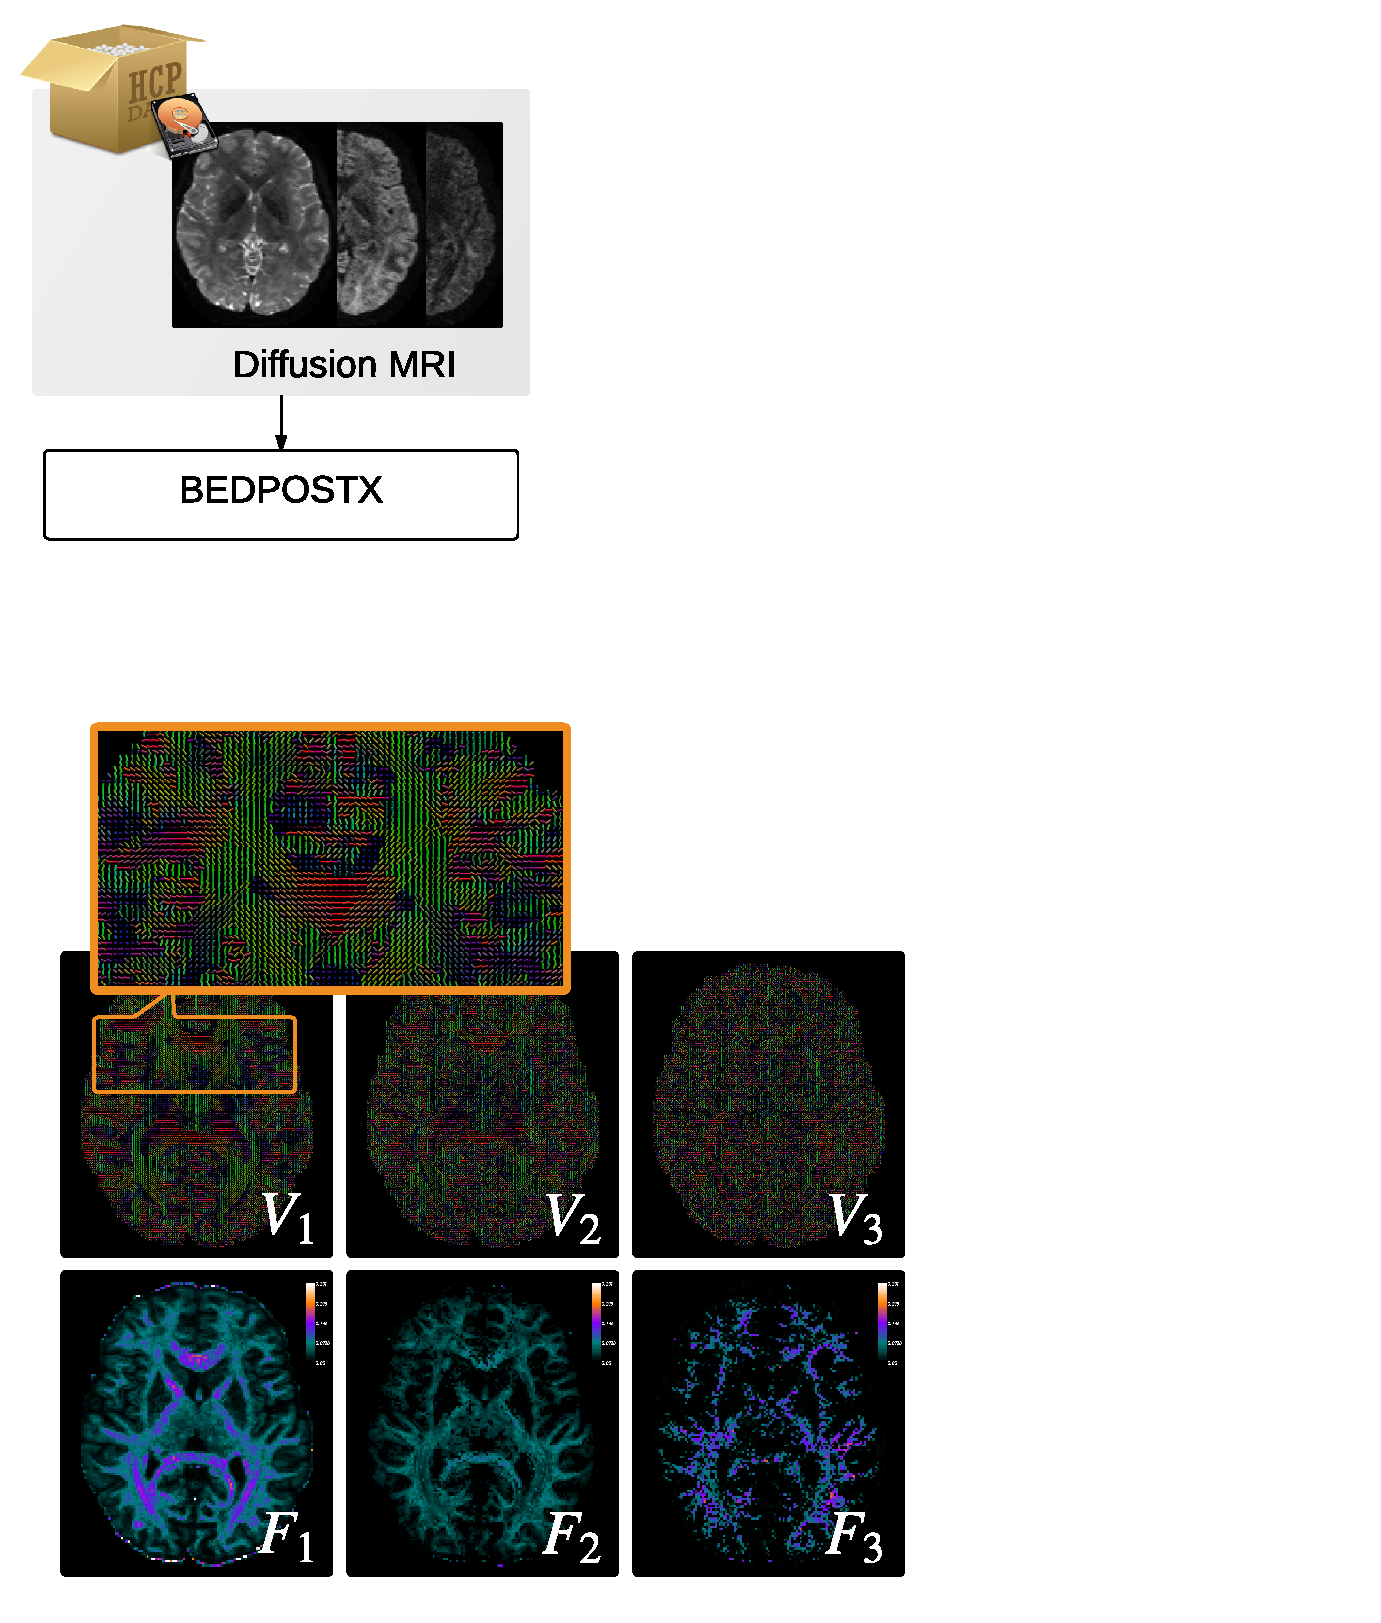
\includegraphics[width=\linewidth]{figures/figure01}
\end{center}
\textbf{\refstepcounter{figure}\label{fig:figure1} Figure \arabic{figure}. }%
{\emph{Diffantom} is a software layer wrapping the \acrfull{hcp} datasets to generate whole-brain diffusion \gls*{dmri} data.
First, the tissue fraction maps $\{T_1, T_2, T_3\}$ are computed using FSL FAST \citep{zhang_segmentation_2001}.
Second, the fiber orientation maps $\{V_1, V_2, V_3\}$ and corresponding volume fraction maps $\{F_1, F_2, F_3\}$ are
  obtained using the ball-and-stick model for multi-shell data of BEDPOSTX \citep{jbabdi_modelbased_2012}.
The third step takes the fiber orientations $\{V_1, V_2, V_3\}$ and their weights $\{F_1, F_2, F_3\}$ to compute the
  corresponding \glspl{fod} using spherical convolution of the single fiber response with each fiber orientation at
  each voxel.
The resulting \glspl{fod} map is then combined with three isotropic compartments corresponding to $\{T_1, T_2, T'_3\}$
  before generating the signal using \emph{phantomas} \citep{caruyer_phantomas_2014}.
The fraction map $T'_3 = T_3 - \sum F_i$ is the remaining isotropic fraction across the \gls*{wm} tissue map.
Finally, data can be used to compute the whole-brain tractography, for instance.}
\end{figure}

\begin{figure}[h!]
\begin{center}
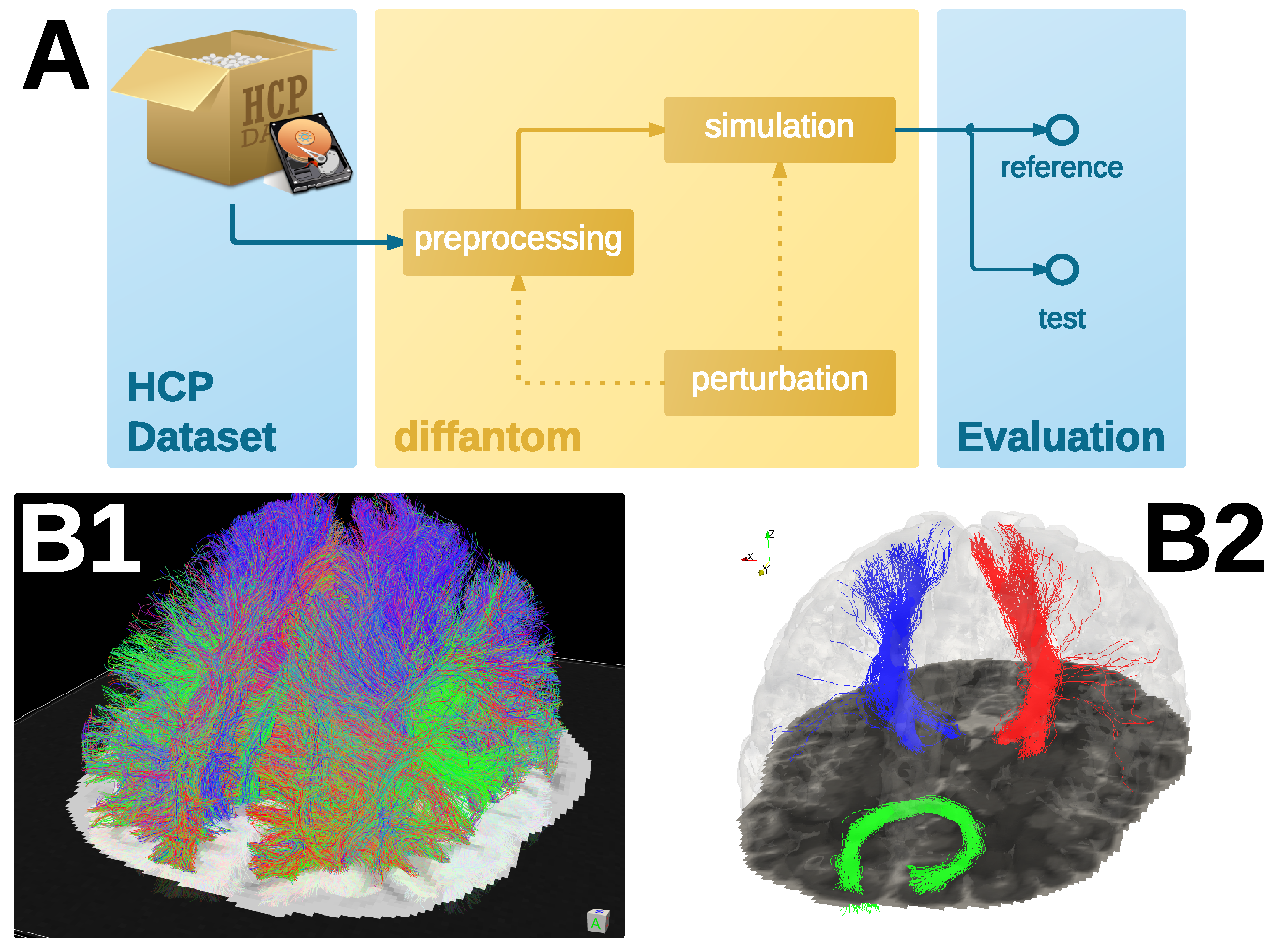
\includegraphics[width=\linewidth]{figures/figure02}
\end{center}
\textbf{\refstepcounter{figure}\label{fig:figure2} Figure \arabic{figure}. }%
{\textbf{A. Recommended use of \emph{diffantom}}.
The dataset can be used to test algorithms and pipelines against a perturbation that is
  introduced in \emph{diffantom}.
Perturbations can model typical artifacts found in \gls*{dmri} datasets or pathological conditions
  such as a tumor.
\textbf{B1, B2, B3. Tractograms of fundamental fiber bundles}.
}
\end{figure}

\end{document}
